\chapter{Analyse et spécification des besoins}

\section*{Introduction}
Après avoir présenté le cadre général du projet dans le premier chapitre, nous abordons maintenant l'analyse du système à développer ainsi que la spécification de ses besoins fonctionnels et non fonctionnels.

\section{Description du système à développer}

Le système proposé vise à développer une application de pé
pinière intelligente permettant de centraliser la gestion des plantes et de leurs informations, d'offrir une plateforme E-commerce pour la consultation et l'achat des plantes, et d'assister les utilisateurs dans le diagnostic de l'état de santé des plantes à partir d'images de leurs plantes. L'application permet également aux gestionnaires de pépinières d'administrer le catalogue de plantes et de suivre les commandes.

\section{Identification des acteurs}

Le tableau suivant présente les différents acteurs de notre système.

\begin{table}[H]
\centering
\renewcommand{\arraystretch}{1.4}
\begin{tabular}{|p{3.2cm}|p{2.3cm}|p{8.5cm}|}
\hline
\textbf{Rôles} & \textbf{Type} & \textbf{Fonctions} \\
\hline
Vendeur & Primaire &
\begin{itemize}
    \item S'authentifier
    \item Gérer plantes
    \item Consulter plantes
    \item Valider commandes
\end{itemize} \\
\hline
Administrateur & Primaire &
\begin{itemize}
    \item Gérer les utilisateurs
    \item Hérite toutes les fonctions du vendeur
\end{itemize} \\
\hline
Client & Primaire &
\begin{itemize}
    \item S'authentifier
    \item Consulter les plantes disponibles à la vente
    \item Ajouter une plante au panier
    \item Passer une commande
    \item Suivre commande
    \item Effectuer diagnostic
\end{itemize} \\
\hline
Module d'assistance au diagnostic et recommandation & Secondaire &
\begin{itemize}
    \item Générer les diagnostics
    \item Générer les recommandations
\end{itemize} \\
\hline
\end{tabular}
\caption{Les différents acteurs du système}
\end{table}

\section{Besoins fonctionnels}

Parmi les besoins fonctionnels que cette application doit couvrir principalement, nous citons :

\subsection*{Client}
Le système doit permettre au client de :
\begin{itemize}
    \item consulter le catalogue des plantes disponibles à la vente ;
    \item ajouter une plante au panier ;
    \item valider le panier et passer une commande ;
    \item suivre ses commandes ;
    \item effectuer un diagnostic de l'état de santé d'une plante à partir d'une image fournie.
\end{itemize}

\subsection*{Vendeur}
Le système doit permettre au vendeur de :
\begin{itemize}
    \item gérer les plantes ;
    \item consulter les plantes ;
    \item valider les commandes des clients.
\end{itemize}

\subsection*{Administrateur}
L'administrateur dispose de l'ensemble des fonctionnalités du vendeur, en plus de la gestion des utilisateurs (clients et vendeurs).

Toutes ces fonctionnalités ne peuvent être réalisées qu'après une authentification.

\subsection*{Module d'assistance au diagnostic et recommandation}
\begin{itemize}
    \item Le système doit intégrer un module d'intelligence artificielle chargé de l'analyse des images des plantes.
    \item Le module IA doit traiter les images envoyées par les clients et retourner un résultat de diagnostic et recommandations.
\end{itemize}

\section{Besoins non fonctionnels}

Les exigences non fonctionnelles visent à garantir la qualité, la fiabilité et l'efficacité de la plateforme de pépinière en ligne, tant sur le plan technique que sur l'expérience utilisateur.

\subsection*{Ergonomie}
\begin{itemize}
    \item L'interface de la plateforme doit être intuitive et facile à utiliser, permettant aux utilisateurs de naviguer aisément entre le catalogue, le panier et le module de diagnostic.
    \item Un design clair et structuré doit faciliter la consultation des plantes et l'accès aux fonctionnalités principales.
\end{itemize}

\subsection*{Performance}
\begin{itemize}
    \item La plateforme doit être capable de gérer simultanément un nombre important d'utilisateurs, de consultations du catalogue et de commandes.
\end{itemize}

\subsection*{Sécurité}
\begin{itemize}
    \item Les données personnelles des utilisateurs (nom, e-mail, informations de compte) doivent être protégées conformément aux normes de sécurité.
    \item Un mécanisme de validation des comptes utilisateurs (vérification de l'e-mail) doit être mis en place afin de limiter les accès frauduleux.
\end{itemize}

\subsection*{Évolutivité}
\begin{itemize}
    \item L'architecture de la plateforme doit permettre l'intégration future de nouvelles fonctionnalités, notamment l'amélioration du système de diagnostic intelligent et de recommandation.
\end{itemize}

\section{Diagramme de cas d'utilisation global}

\begin{figure}[H]
    \centering
    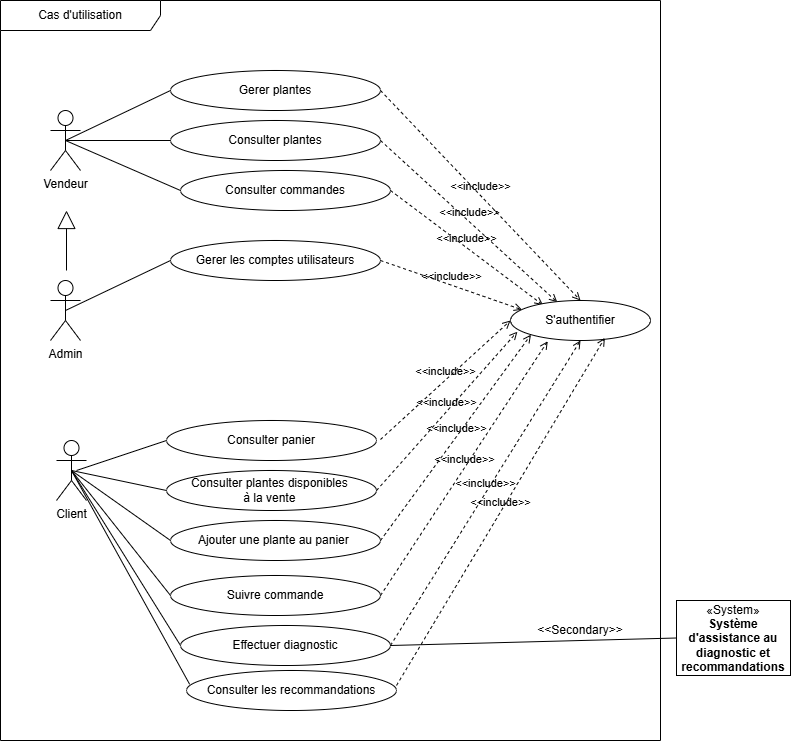
\includegraphics[width=0.85\textwidth]{images/CasUtilisation.png}
    \caption{Diagramme de cas d'utilisation global}
\end{figure}

\section{Raffinement des cas d'utilisation}

\subsection{Cas d'utilisation << Gérer plante >>}

Ce cas d'utilisation permet au vendeur ou à l'administrateur de modifier le stock, modifier, supprimer et ajouter une plante.
cette \autoref{fig:figure1} représente le raffinement de cas d'utilisation << Gérer plante >>.

\begin{figure}[H]
    \centering
    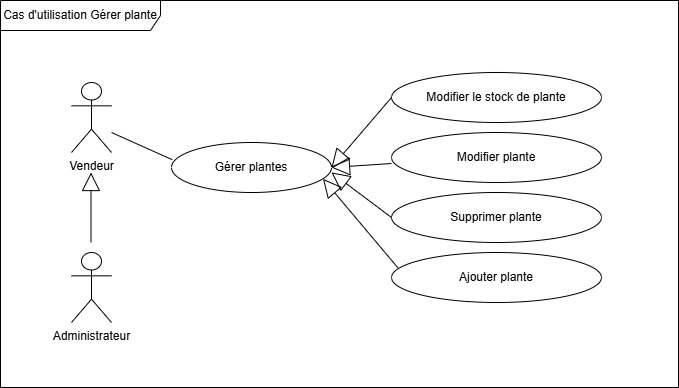
\includegraphics[width=0.75\textwidth]{images/gerer plante2.png}
    \caption{Raffinement du cas d'utilisation « Gérer plante »}
    \label{fig:figure1}
\end{figure}

\subsubsection{Cas d'utilisation << Modifier le stock d'une plante>>}

Le tableau présente la description textuelle du cas d'utilisation « Modifier le stock d'une plante».

\begin{table}[H]
\centering
\renewcommand{\arraystretch}{1.4}
\begin{tabular}{|p{4cm}|p{10cm}|}
\hline
\textbf{Titre} & Modifier le stock d'une plante \\
\hline
\textbf{Acteur} & Vendeur, Administrateur \\
\hline
\textbf{Résumé} & Cas d'utilisation permettant à un vendeur ou à un administrateur de modifier le stock d'une plante. \\
\hline
\textbf{Préconditions} &
\begin{itemize}
    \item Client authentifié.
    \item Plante existe déjà.
\end{itemize} \\
\hline
\textbf{Postconditions} &
\begin{itemize}
    \item Quantité de plantes est mise à jour dans la base de données.
    \item La plante est disponible à la vente.
\end{itemize} \\
\hline
\textbf{Scénario nominal} &
\begin{enumerate}
    \item Le vendeur/administrateur accède à l'interface de gestion des plantes.
    \item Le système affiche la liste des plantes.
    \item L'acteur sélectionne la plante à modifier.
    \item Le système affiche les détails de la plante, y compris la quantité en stock actuelle.
    \item L'acteur saisit la nouvelle quantité en stock.
    \item L'acteur valide la modification.
    \item Le système vérifie la validité des données saisies.
    \item Le système met à jour la quantité en stock dans la base de données et affiche un message de confirmation.
\end{enumerate} \\
\hline
\textbf{Enchaînements d'erreurs} &
\textbf{E1 : Quantité invalide}
\begin{itemize}
    \item À l'étape 5 du scénario nominal, l'acteur saisit une valeur négative ou non numérique.
    \item Le système affiche un message d'erreur et le cas d'utilisation est terminé.
\end{itemize} \\
\hline
\end{tabular}
\caption{Cas d'utilisation « Modifier le stock d'une plante»}
\end{table}

\subsubsection{Cas d'utilisation << Modifier plante >>}

Le tableau présente la description textuelle du cas d'utilisation « Modifier plante ».

\begin{table}[H]
\centering
\renewcommand{\arraystretch}{1.4}
\begin{tabular}{|p{4cm}|p{10cm}|}
\hline
\textbf{Titre} & Modifier plante \\
\hline
\textbf{Acteur} & Vendeur, Administrateur \\
\hline
\textbf{Résumé} & Cas d'utilisation permettant à un vendeur ou à un administrateur de modifier une plante. \\
\hline
\textbf{Préconditions} &
\begin{itemize}
    \item Client authentifié.
    \item Plante existe déjà.
\end{itemize} \\
\hline
\textbf{Postconditions} &
\begin{itemize}
    \item Les données de la plante sont mises à jour.
\end{itemize} \\
\hline
\textbf{Scénario nominal} &
\begin{enumerate}
    \item L'acteur accède à l'interface de gestion des plantes.
    \item Le système affiche la liste des plantes.
    \item L'acteur sélectionne la plante à modifier.
    \item Le système affiche les informations actuelles de la plante.
    \item L'acteur modifie les champs souhaités et valide les modifications.
    \item Le système vérifie la validité des données saisies et enregistre les modifications.
    \item Le système affiche un message de confirmation.
\end{enumerate} \\
\hline
\end{tabular}
\caption{Cas d'utilisation « Modifier plante »}
\end{table}

\subsubsection{Cas d'utilisation << Ajouter plante >>}

Le tableau présente la description textuelle du cas d'utilisation « Ajouter plante ».

\begin{table}[H]
\centering
\renewcommand{\arraystretch}{1.4}
\begin{tabular}{|p{4cm}|p{10cm}|}
\hline
\textbf{Titre} & Ajouter plante \\
\hline
\textbf{Acteur} & Vendeur, Administrateur \\
\hline
\textbf{Résumé} & Cas d'utilisation permettant à un vendeur ou à un administrateur d'ajouter une plante. \\
\hline
\textbf{Préconditions} &
\begin{itemize}
    \item Client authentifié.
\end{itemize} \\
\hline
\textbf{Scénario nominal} &
\begin{enumerate}
    \item L'acteur accède à l'interface de gestion des plantes et clique sur « Ajouter plante ».
    \item Le système affiche le formulaire d'ajout.
    \item L'acteur saisit les informations de la plante et valide le formulaire.
    \item Le système vérifie la validité des données saisies.
    \item Le système enregistre la plante et affiche un message de confirmation.
\end{enumerate} \\
\hline
\textbf{Enchaînements alternatifs} &
\textbf{A1 : L'acteur laisse un champ vide}
\begin{itemize}
    \item À l'étape 4, le système affiche une alerte et l'acteur doit reprendre à l'étape 3.
\end{itemize} \\
\hline
\textbf{Scénario d'erreur} &
\textbf{E1 : Plante déjà existante}
\begin{itemize}
    \item À l'étape 4, le système affiche une alerte et l'acteur doit reprendre à l'étape 3.
\end{itemize} \\
\hline
\end{tabular}
\caption{Cas d'utilisation « Ajouter plante »}
\end{table}

\subsubsection{Cas d'utilisation << Supprimer plante >>}

Le tableau présente la description textuelle du cas d'utilisation « Supprimer plante ».

\begin{table}[H]
\centering
\renewcommand{\arraystretch}{1.4}
\begin{tabular}{|p{4cm}|p{10cm}|}
\hline
\textbf{Titre} & Supprimer plante \\
\hline
\textbf{Acteur} & Vendeur, Administrateur \\
\hline
\textbf{Résumé} & Cas d'utilisation permettant à un vendeur ou à un administrateur de supprimer une plante. \\
\hline
\textbf{Préconditions} &
\begin{itemize}
    \item Client authentifié.
    \item Plante existe déjà.
\end{itemize} \\
\hline
\textbf{Postconditions} & La plante n'est plus visible sur le site. \\
\hline
\textbf{Scénario nominal} &
\begin{enumerate}
    \item L'acteur accède à l'interface de gestion des plantes.
    \item Le système affiche la liste des plantes.
    \item L'acteur sélectionne la plante à supprimer et clique sur supprimer.
    \item Le système demande une confirmation de suppression.
    \item L'acteur confirme l'opération.
    \item Le système supprime la plante de la base de données et affiche un message de confirmation.
\end{enumerate} \\
\hline
\end{tabular}
\caption{Cas d'utilisation « Supprimer plante »}
\end{table}

\subsection{Cas d'utilisation << Consulter plantes >>}

Ce cas d'utilisation permet au vendeur de consulter la liste des plantes.

\begin{figure}[H]
    \centering
    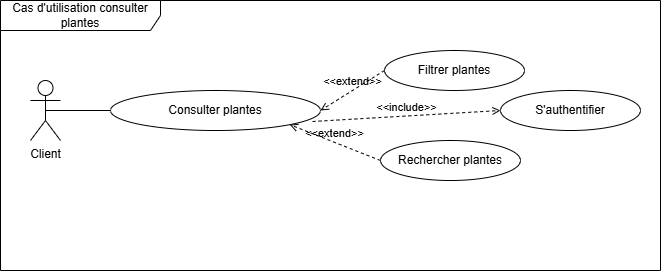
\includegraphics[width=0.75\textwidth]{images/consulter plantes.png}
    \caption{Raffinement du cas d'utilisation « Consulter plantes »}
\end{figure}

\begin{table}[H]
\centering
\renewcommand{\arraystretch}{1.4}
\begin{tabular}{|p{4cm}|p{10cm}|}
\hline
\textbf{Titre} & Consulter plantes \\
\hline
\textbf{Acteur} & Vendeur \\
\hline
\textbf{Résumé} & Cas d'utilisation permettant au vendeur d'accéder à la liste des plantes. \\
\hline
\textbf{Préconditions} &
\begin{itemize}
    \item Vendeur authentifié.
    \item Plantes enregistrées dans la base de données.
\end{itemize} \\
\hline
\textbf{Postconditions} & Liste des plantes affichée. \\
\hline
\textbf{Scénario nominal} &
\begin{enumerate}
    \item Le vendeur accède à la section « Plantes ».
    \item Le système affiche la liste des plantes disponibles.
\end{enumerate} \\
\hline
\textbf{Scénario alternatif} &
\textbf{A1 : Filtrer les plantes}
\begin{itemize}
    \item À l'étape 2, le vendeur choisit de filtrer les plantes selon un des critères suivants (plante d'intérieur, d'extérieur, prix, besoin en lumière, eau, température...).
    \item Le système reprend à l'étape 2.
\end{itemize}

\textbf{A2 : Rechercher une plante}
\begin{itemize}
    \item À l'étape 2, le vendeur choisit de rechercher une plante en tapant un mot clé.
    \item Le système reprend à l'étape 2.
\end{itemize} \\
\hline
\end{tabular}
\caption{Cas d'utilisation « Consulter plantes »}
\end{table}

\subsection{Cas d'utilisation << Consulter commandes >>}

Le tableau présente la description textuelle du cas d'utilisation « Consulter commandes ».

\begin{figure}[H]
    \centering
    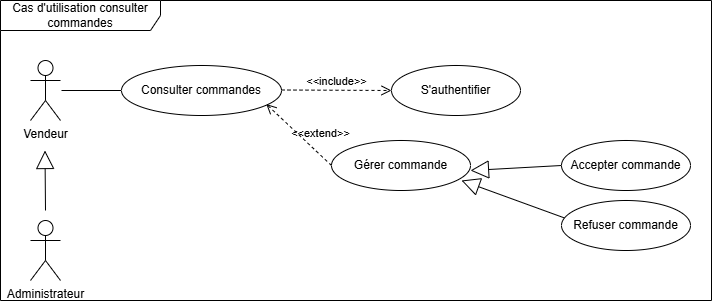
\includegraphics[width=0.75\textwidth]{images/consulter commandes.png}
    \caption{Raffinement du cas d'utilisation « Consulter commandes »}
\end{figure}

\begin{table}[H]
\centering
\renewcommand{\arraystretch}{1.4}
\begin{tabular}{|p{4cm}|p{10cm}|}
\hline
\textbf{Titre} & Consulter commandes \\
\hline
\textbf{Acteur} & Vendeur, Administrateur \\
\hline
\textbf{Résumé} & Cas d'utilisation permettant au vendeur ainsi qu'à l'administrateur d'accéder à la liste des commandes. \\
\hline
\textbf{Préconditions} &
\begin{itemize}
    \item Acteur authentifié.
    \item Commandes enregistrées.
\end{itemize} \\
\hline
\textbf{Postconditions} & Liste des commandes affichée. \\
\hline
\textbf{Scénario nominal} &
\begin{enumerate}
    \item L'acteur accède à la section « Commandes ».
    \item Le système affiche la liste des commandes.
\end{enumerate} \\
\hline
\textbf{Scénario alternatif} &
\textbf{A1 : Recherche d'un compte utilisateur}
\begin{itemize}
    \item À l'étape 2, l'administrateur choisit de faire une recherche, il saisit un mot-clé (nom, email...).
    \item Le système affiche les comptes correspondants.
\end{itemize}

\textbf{A2 : Filtrage des comptes utilisateurs}
\begin{itemize}
    \item À l'étape 2, l'administrateur choisit d'appliquer un filtre selon un des critères suivants (statut actif/désactivé, rôle client/vendeur...).
    \item Le système met à jour la liste affichée.
\end{itemize} \\
\hline
\end{tabular}
\caption{Cas d'utilisation « Consulter commandes »}
\end{table}

\subsection{Cas d'utilisation << Gérer commandes >>}

Ce cas d'utilisation permet au vendeur ainsi qu'à l'administrateur de gérer les commandes passées par les clients.

\begin{figure}[H]
    \centering
    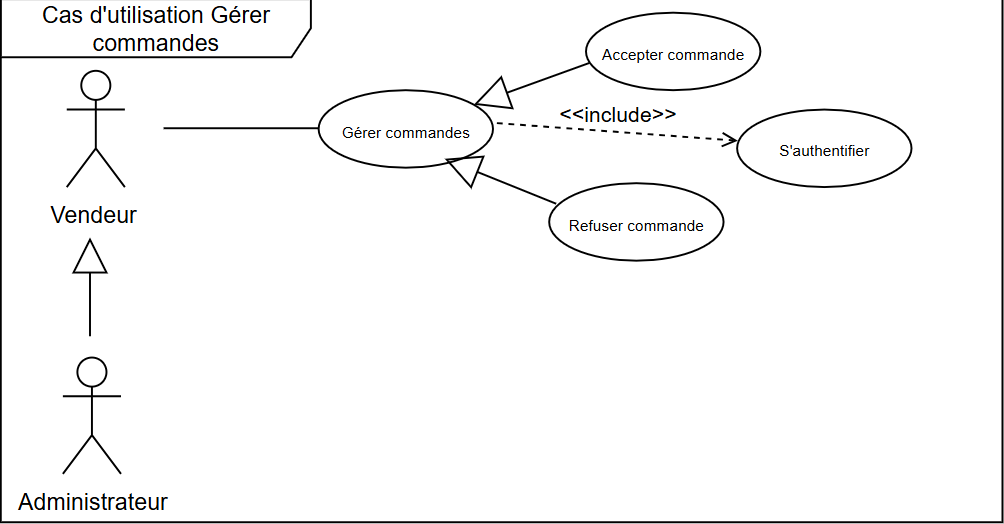
\includegraphics[width=0.75\textwidth]{images/gérer commandes.png}
    \caption{Raffinement du cas d'utilisation « Gérer commandes »}
\end{figure}

\subsubsection{Cas d'utilisation << Accepter commande >>}

Le tableau présente la description textuelle du cas d'utilisation « Accepter commande ».

\begin{table}[H]
\centering
\renewcommand{\arraystretch}{1.4}
\begin{tabular}{|p{4cm}|p{10cm}|}
\hline
\textbf{Titre} & Accepter commande \\
\hline
\textbf{Acteur} & Vendeur, Administrateur \\
\hline
\textbf{Résumé} & Cas d'utilisation permettant au vendeur ainsi qu'à l'administrateur d'accepter une commande. \\
\hline
\textbf{Préconditions} &
\begin{itemize}
    \item Acteur authentifié.
    \item Commande avec statut « En attente ».
\end{itemize} \\
\hline
\textbf{Postconditions} & Statut de la commande mis à « Acceptée ». \\
\hline
\textbf{Scénario nominal} &
\begin{enumerate}
    \item L'acteur sélectionne une commande en attente.
    \item Le système affiche les détails de la commande.
    \item L'acteur clique sur « Accepter ».
    \item Le système vérifie la disponibilité du stock.
    \item Le système met à jour le statut de la commande et affiche un message de confirmation.
\end{enumerate} \\
\hline
\textbf{Scénario d'erreur} &
\textbf{E1 : Validation abandonnée}
\begin{itemize}
    \item À l'étape 3, l'acteur décide d'annuler l'opération.
    \item Le système ne modifie pas la commande et le cas d'utilisation se termine.
\end{itemize}

\textbf{E2 : Stock insuffisant}
\begin{itemize}
    \item À l'étape 4, le système détecte que la quantité demandée n'est plus disponible.
    \item Le système affiche un message d'erreur.
\end{itemize} \\
\hline
\end{tabular}
\caption{Cas d'utilisation « Accepter commande »}
\end{table}

\subsubsection{Cas d'utilisation << Refuser commande >>}

Le tableau présente la description textuelle du cas d'utilisation « Refuser commande ».

\begin{table}[H]
\centering
\renewcommand{\arraystretch}{1.4}
\begin{tabular}{|p{4cm}|p{10cm}|}
\hline
\textbf{Titre} & Refuser commande \\
\hline
\textbf{Acteur} & Vendeur, Administrateur \\
\hline
\textbf{Résumé} & Cas d'utilisation permettant au vendeur ainsi qu'à l'administrateur de refuser une commande. \\
\hline
\textbf{Préconditions} &
\begin{itemize}
    \item Acteur authentifié.
    \item Commande avec statut « En attente ».
\end{itemize} \\
\hline
\textbf{Postconditions} & Statut de la commande mis à « Refusée ». \\
\hline
\textbf{Scénario nominal} &
\begin{enumerate}
    \item L'acteur sélectionne une commande en attente.
    \item Le système affiche les détails de la commande.
    \item L'acteur clique sur « Refuser ».
    \item Le système met à jour le statut de la commande et affiche un message de confirmation.
\end{enumerate} \\
\hline
\textbf{Scénario d'erreur} &
\textbf{E1 : Refus abandonné}
\begin{itemize}
    \item À l'étape 3, l'acteur décide d'annuler l'opération.
    \item Le système ne modifie pas la commande et le cas d'utilisation se termine.
\end{itemize} \\
\hline
\end{tabular}
\caption{Cas d'utilisation « Refuser commande »}
\end{table}

\subsection{Cas d'utilisation << Gérer comptes utilisateurs >>}

Ce cas d'utilisation permet à l'administrateur de gérer les comptes utilisateurs.

\begin{figure}[H]
    \centering
    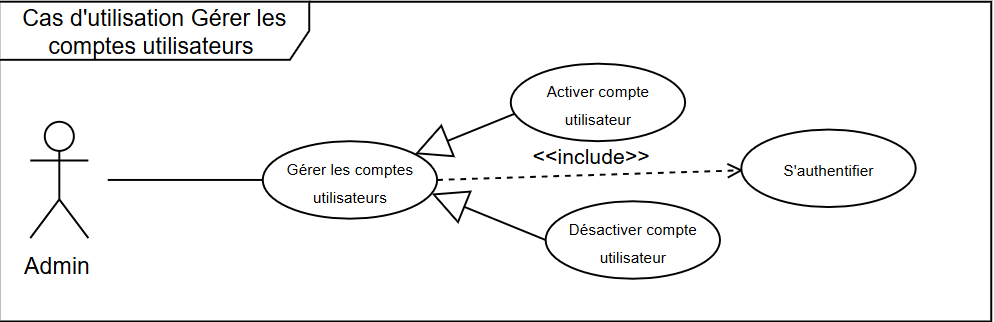
\includegraphics[width=0.75\textwidth]{images/gérer comptes utilisateurs.png}
    \caption{Raffinement du cas d'utilisation « Gérer comptes utilisateurs »}
\end{figure}

\subsubsection{Cas d'utilisation << Activer compte utilisateur >>}

Le tableau présente la description textuelle du cas d'utilisation « Activer compte utilisateur ».

\begin{table}[H]
\centering
\renewcommand{\arraystretch}{1.4}
\begin{tabular}{|p{4cm}|p{10cm}|}
\hline
\textbf{Titre} & Activer compte utilisateur \\
\hline
\textbf{Acteur} & Administrateur \\
\hline
\textbf{Résumé} & Cas d'utilisation permettant à l'administrateur d'activer un compte utilisateur afin de lui permettre d'accéder aux fonctionnalités de la plateforme. \\
\hline
\textbf{Préconditions} &
\begin{itemize}
    \item Administrateur authentifié.
    \item Compte avec statut « En attente ».
\end{itemize} \\
\hline
\textbf{Postconditions} & Compte utilisateur activé. \\
\hline
\textbf{Scénario nominal} &
\begin{enumerate}
    \item L'administrateur sélectionne un compte dont le statut est « En attente ».
    \item Le système affiche les détails du compte.
    \item L'administrateur clique sur « Activer ».
    \item Le système met à jour le statut du compte et affiche un message de succès.
\end{enumerate} \\
\hline
\end{tabular}
\caption{Cas d'utilisation « Activer compte utilisateur »}
\end{table}

\subsubsection{Cas d'utilisation << Désactiver compte utilisateur >>}

Le tableau présente la description textuelle du cas d'utilisation « Désactiver compte utilisateur ».

\begin{table}[H]
\centering
\renewcommand{\arraystretch}{1.4}
\begin{tabular}{|p{4cm}|p{10cm}|}
\hline
\textbf{Titre} & Désactiver compte utilisateur \\
\hline
\textbf{Acteur} & Administrateur \\
\hline
\textbf{Résumé} & Cas d'utilisation permettant à l'administrateur de suspendre temporairement un compte utilisateur. \\
\hline
\textbf{Préconditions} &
\begin{itemize}
    \item Administrateur authentifié.
    \item Compte actif.
\end{itemize} \\
\hline
\textbf{Postconditions} & Compte utilisateur désactivé. \\
\hline
\textbf{Scénario nominal} &
\begin{enumerate}
    \item L'administrateur sélectionne un compte actif.
    \item Le système affiche les détails du compte.
    \item L'administrateur clique sur « Désactiver ».
    \item Le système met à jour le statut du compte et affiche un message de succès.
\end{enumerate} \\
\hline
\end{tabular}
\caption{Cas d'utilisation « Désactiver compte utilisateur »}
\end{table}

\subsection{Cas d'utilisation << Consulter comptes utilisateurs >>}

Le tableau présente la description textuelle du cas d'utilisation « Consulter comptes utilisateurs ».

\begin{figure}[H]
    \centering
    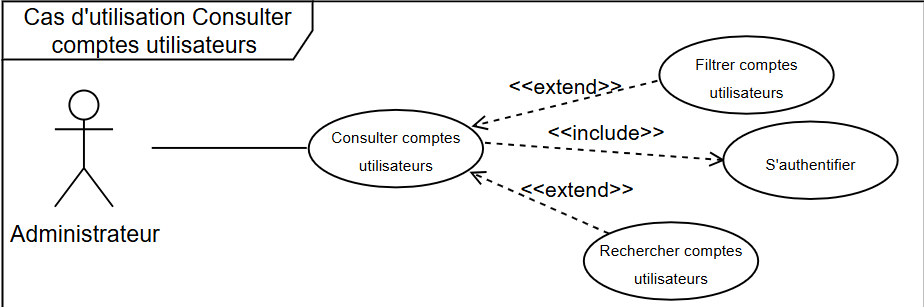
\includegraphics[width=0.75\textwidth]{images/consulter comptes utilisateurs.png}
    \caption{Raffinement du cas d'utilisation « Consulter comptes utilisateurs »}
\end{figure}

\begin{table}[H]
\centering
\renewcommand{\arraystretch}{1.4}
\begin{tabular}{|p{4cm}|p{10cm}|}
\hline
\textbf{Titre} & Consulter comptes utilisateurs \\
\hline
\textbf{Acteur} & Administrateur \\
\hline
\textbf{Résumé} & Cas d'utilisation permettant à l'administrateur d'accéder à la liste des comptes utilisateurs. \\
\hline
\textbf{Préconditions} &
\begin{itemize}
    \item Administrateur authentifié.
    \item Comptes utilisateurs existants.
\end{itemize} \\
\hline
\textbf{Postconditions} & Liste des comptes utilisateurs affichée. \\
\hline
\textbf{Scénario nominal} &
\begin{enumerate}
    \item L'administrateur accède à la section « Comptes utilisateurs ».
    \item Le système affiche la liste des comptes avec leurs informations principales et leur statut.
\end{enumerate} \\
\hline
\textbf{Scénario alternatif} &
\textbf{A1 : Recherche d'un compte utilisateur}
\begin{itemize}
    \item À l'étape 2, l'administrateur saisit un mot-clé (nom, email...).
    \item Le système affiche les comptes correspondants.
\end{itemize}

\textbf{A2 : Filtrage des comptes utilisateurs}
\begin{itemize}
    \item À l'étape 2, l'administrateur applique un filtre (statut actif/désactivé, rôle client/vendeur...).
    \item Le système met à jour la liste affichée.
\end{itemize} \\
\hline
\end{tabular}
\caption{Cas d'utilisation « Consulter comptes utilisateurs »}
\end{table}

\subsubsection{Cas d'utilisation << Consulter panier >>}
\begin{figure}[H]
    \centering
    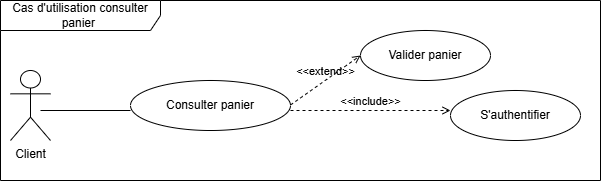
\includegraphics[width=0.75\textwidth]{images/Consulter panier.png}
    \caption{Raffinement du cas d'utilisation « Consulter panier »}
\end{figure}


Le tableau présente la description textuelle du cas d'utilisation « Consulter panier ».

\begin{table}[H]
\centering
\renewcommand{\arraystretch}{1.4}
\begin{tabular}{|p{4cm}|p{10cm}|}
\hline
\textbf{Titre} & Consulter panier \\
\hline
\textbf{Acteur} & Client \\
\hline
\textbf{Résumé} & Cas d'utilisation permettant au client de consulter son panier \\
\hline
\textbf{Préconditions} &
\begin{itemize}
    \item Client authentifié.
    \item Panier existe
\end{itemize} \\
\hline
\textbf{Postconditions} & Liste des plantes dans le panier affichés. \\
\hline
\textbf{Scénario nominal} &
\begin{enumerate}
    \item Le client clique sur le panier.
    \item Le système affiche la liste des plantes que le client a ajouté dans le panier.
\end{enumerate} \\
\hline
\end{tabular}
\caption{Cas d'utilisation « Activer compte utilisateur »}
\end{table}

\subsection{Cas d'utilisation << Ajouter une plante au panier >>}

\begin{table}[H]
\centering
\renewcommand{\arraystretch}{1.4}
\begin{tabular}{|p{4cm}|p{10cm}|}
\hline
\textbf{Titre} & Ajouter une plante au panier \\
\hline
\textbf{Acteur} & Client \\
\hline
\textbf{Résumé} & Cas d'utilisation permettant au client d'ajouter une plante sélectionnée à son panier afin de préparer une commande. \\
\hline
\textbf{Préconditions} &
\begin{itemize}
    \item Client authentifié.
    \item Plante disponible à la vente.
\end{itemize} \\
\hline
\textbf{Postconditions} & Plante ajoutée au panier du client. \\
\hline
\textbf{Scénario nominal} &
\begin{enumerate}
    \item Le client consulte la liste des plantes disponibles.
    \item Il sélectionne une plante.
    \item Il choisit la quantité souhaitée.
    \item Il clique sur « Ajouter au panier ».
    \item Le système enregistre la plante dans le panier et affiche un message de confirmation.
\end{enumerate} \\
\hline
\textbf{Scénario alternatif} &
\textbf{A1 : Modification de la quantité}
\begin{itemize}
    \item À l'étape 3, le client modifie la quantité avant la confirmation.
    \item Le système prend en compte la nouvelle quantité.
\end{itemize} \\
\hline
\end{tabular}
\caption{Cas d'utilisation « Ajouter une plante au panier »}
\end{table}

\subsection{Cas d'utilisation << Passer une commande >>}

Le tableau présente la description textuelle du cas d'utilisation « Passer une commande ».

\begin{table}[H]
\centering
\renewcommand{\arraystretch}{1.4}
\begin{tabular}{|p{4cm}|p{10cm}|}
\hline
\textbf{Titre} & Passer une commande \\
\hline
\textbf{Acteur} & Client \\
\hline
\textbf{Résumé} & Cas d'utilisation permettant à un client de passer une commande. \\
\hline
\textbf{Préconditions} &
\begin{itemize}
    \item Client authentifié.
    \item Plante disponible à la vente.
\end{itemize} \\
\hline
\textbf{Postconditions} &
\begin{itemize}
    \item Stock mis à jour.
    \item Reçu de la commande.
\end{itemize} \\
\hline
\textbf{Scénario nominal} &
\begin{enumerate}
    \item Le client choisit une plante.
    \item Les détails de la plante sont affichés.
    \item Le client ajoute la plante au panier.
    \item La fiche des coordonnées est affichée.
    \item Le client remplit la fiche avec ses coordonnées.
    \item Le reçu de la commande est affiché.
\end{enumerate} \\
\hline
\textbf{Scénario alternatif} &
\textbf{A1 : Le client décide de quitter la page}
\begin{itemize}
    \item À l'étape 3, le client décide de quitter la page.
    \item Le système affiche la liste des plantes.
    \item Le client est invité de recommencer à l'étape 1.
\end{itemize} \\
\hline
\end{tabular}
\caption{Cas d'utilisation « Passer une commande »}
\end{table}

\subsection{Cas d'utilisation << Suivre commande >>}

Le tableau présente la description textuelle du cas d'utilisation « Suivre commande ».

\begin{table}[H]
\centering
\renewcommand{\arraystretch}{1.4}
\begin{tabular}{|p{4cm}|p{10cm}|}
\hline
\textbf{Titre} & Suivre commande \\
\hline
\textbf{Acteur} & Client \\
\hline
\textbf{Résumé} & Cas d'utilisation permettant au client de suivre l'état de sa commande. \\
\hline
\textbf{Préconditions} &
\begin{itemize}
    \item Client authentifié.
    \item Commande créée.
\end{itemize} \\
\hline
\textbf{Postconditions} & L'état de la commande est affiché. \\
\hline
\textbf{Scénario nominal} &
\begin{enumerate}
    \item Le client clique sur la commande.
    \item Le système affiche l'état de la commande.
\end{enumerate} \\
\hline
\end{tabular}
\caption{Cas d'utilisation « Suivre commande »}
\end{table}

\subsection{Cas d'utilisation << Effectuer diagnostic >>}

Le tableau présente la description textuelle du cas d'utilisation « Effectuer diagnostic ».

\begin{table}[H]
\centering
\renewcommand{\arraystretch}{1.4}
\begin{tabular}{|p{4cm}|p{10cm}|}
\hline
\textbf{Titre} & Effectuer diagnostic \\
\hline
\textbf{Acteur} & Client, Module d'assistance au diagnostic \\
\hline
\textbf{Résumé} & Cas d'utilisation permettant au client de diagnostiquer sa plante et recevoir des recommandations. \\
\hline
\textbf{Préconditions} &
\begin{itemize}
    \item Client authentifié.
\end{itemize} \\
\hline
\textbf{Postconditions} & Le diagnostic de la plante et les recommandations sont affichées. \\
\hline
\textbf{Scénario nominal} &
\begin{enumerate}
    \item Le client clique sur le menu « Diagnostic ».
    \item Le système affiche un champ de chargement d'une photo.
    \item Le client charge la photo de la plante.
    \item Le système analyse l'image chargée.
    \item Le système affiche les diagnostics avec des recommandations.
\end{enumerate} \\
\hline
\textbf{Scénario d'erreur} &
\textbf{E1 : Photo non exploitable}
\begin{itemize}
    \item À l'étape 5, le système affiche un message d'erreur indiquant que la photo est inexploitable.
    \item Le système redemande au client de charger une nouvelle photo.
\end{itemize} \\
\hline
\end{tabular}
\caption{Cas d'utilisation « Effectuer diagnostic »}
\end{table}

\section*{Conclusion}

Après avoir présenté le système à développer, identifié les différents acteurs et réalisé l'analyse fonctionnelle ainsi que l'étude des besoins non fonctionnels, le chapitre suivant sera consacré à la conception générale et détaillée de la solution proposée.